\documentclass[conference]{./IEEEtran}

\usepackage{cite}
\usepackage[pdftex]{graphicx}
\usepackage{algorithmic}

% correct bad hyphenation here
\hyphenation{op-tical net-works semi-conduc-tor}


\begin{document}

\title{Conductor.....}

\author{\IEEEauthorblockN{Davide Pesavento}
\IEEEauthorblockA{Universit\`{a} degli Studi di Padova\\
Corso di Laurea Magistrale in Informatica\\
Email: email@studenti.math.unipd.it}
\and
\IEEEauthorblockN{Martina Astegno}
\IEEEauthorblockA{Universit\`{a} degli Studi di Padova\\
Corso di Laurea Magistrale in Informatica\\
Email: martina.astegno@studenti.unipd.it}}

% make the title area
\maketitle


\begin{abstract}
%\boldmath
We present in this paper an application that shows how the bluetooth technology can be used to locate a person who has a bluetooth device (e.g. smartphone) in a set of possible rooms.  The final aim is to playback an audio stream stored in a central server and move it from a speaker to an another, situated in every room, following person's movements.
\end{abstract}
% IEEEtran.cls defaults to using nonbold math in the Abstract.
% This preserves the distinction between vectors and scalars. However,
% if the conference you are submitting to favors bold math in the abstract,
% then you can use LaTeX's standard command \boldmath at the very start
% of the abstract to achieve this. Many IEEE journals/conferences frown on
% math in the abstract anyway.

\begin{IEEEkeywords}%normally used for peerreview paper
Bluetooth, Pulseaudio, conductor.
\end{IEEEkeywords}




% For peer review papers, you can put extra information on the cover
% page as needed:
% \ifCLASSOPTIONpeerreview
% \begin{center} \bfseries EDICS Category: 3-BBND \end{center}
% \fi
%
% For peerreview papers, this IEEEtran command inserts a page break and
% creates the second title. It will be ignored for other modes.
\IEEEpeerreviewmaketitle


%\hfill October 16, 2010

\section{Introduction}
In 1994 L.M. Ericsson company began to be interested in wireless connection between cellular phones and other devices. With other four companies it formed a group, SIG, to develop a new standard wireless used to link computation and communication devices throught a wireless radio system with low costs, restricted power and range. The project was called Bluetooth and after five years it was published the first version 1.0 specific.
In figure \ref{stack} we can see the architecture of bluetooth protocol.
\begin{figure}[h]
\centering
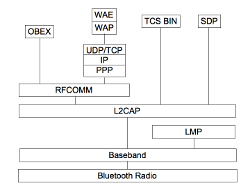
\includegraphics[scale = 0.8]{stacksimple1.png}
\caption{Bluetooth Protocol Stack}
\label{stack}
\end{figure}

The protocols can be divided in four major classes:
\begin{itemize}
\item Core protocols
\item Cable replacement protocols
\item Telephony control protocols
\item Adopted protocols
\end{itemize}

%-------TOFIX: a questo punto pesanvo di concertrare l'attenzione sul service discovery protocol usato per individuare le altre devices.e spiegare u pò come funzia


%The bluetooth protocol acts in 2.4Ghz frequency using 79 channels (between 2.402 and 2.480 Ghz) and the maximum transmission velocity is 2.1 Mbit/s (version 2.0). The devices can be divided in three classes according to power level and range.\\
%dopo un intro alla tecnologia del bluetooth introduco un pò coem viene gestito il flusso audio con pulseaudio server e così finisce l'intro-----------
\section{General architecture}
\subsection{Requirements}
The requirements for the correct functioning of the implemented application can be explained to follow.
\begin{itemize}
\item{\textbf{Smartphone:}} the device necessary to locate in which room the person is. We assume that there is only one smartphone to identify.  
\item{\textbf{Central server:}} it stores the main application and it controls all the communications from/to the BT adapter.
\end{itemize}
In every room there must be available:
\begin{itemize}
\item{a \textbf{bluetooth host adapter:}} it detects the bluetooth signal power, and trasmits throught a simple application the RSSI value to the central server; 
\item{a \textbf{speaker:}} it lets out sound when the associate BT adapter is selected for playback.
\end{itemize}

%immagine con la architettura ad alto livello che mostra come interagiscono le componenti

\subsection{Bluetooth module}
The main component of the project is the Bluetooth module, that manages the RSSI values and communications between hosts and server. It is based on a simple and very efficient application, named \texttt{Probe} and associated to every bleutooth adapter, that is able to interface with \textbf{bluez} throught \textbf{d-bus}. It takes charge of a discovery request and it keeps track of adapters available and their corresponding RSSI values.     

\subsection{Pulseaudio module}
In Pulseaudio we distinguish two particolar types of structures managed in our application.
\begin{itemize}
\item \texttt{pa\_sink}: it rapresents
\item \texttt{pa\_sink\_input}:
\end{itemize}
The idea concerns in redirecting the \texttt{pa\_sink\_input} coming from a specific application (e.g. MPlayer) to one or more \texttt{pa\_sink} associated with a speaker in every room.
By default the audio is reproduced by only one \texttt{pa\_sink}, but according to needs, it's possible to playback sound from more speakers simultaneously.
\subsection{Algorithm}
The algorithm implemented determines which speaker has to playback sound according to person's location; we can suppose infact that the signal power detected by the bluetooth adapter is higher than the other RSSI values in the room where person is situated. The following pseudo-code shows how the algorithm works. The output returned represents the index of speakers/rooms where the sound has to be reproduced.

Input variables:
\begin{itemize}
\item \textbf{Defer\_count}: time spent from inizialization to the request of available RSSI.
\item \textbf{Expiry\_time}: if this threshold is exceeded the playback is forced to start, even if there aren't all data available. 
\item \textbf{Current\_room}: location of the person in the current moment.
\item \textbf{No\_null\_RSSI}: number of available RSSI values.
\item \textbf{Adjacences\_map}: stores the adjacences between different rooms.
\item \textbf{RSSI\_map}: associates to every BT adapter the RSSI value detected.
\item \textbf{Min\_number\_RSSI}: min number of RSSI required to proceed with the sound playback. 
\item \textbf{Max\_number\_speakers}: max number of speakers that can be activated simultanously.
\end{itemize}
\textbf{\underline{Choice algorithm:}}
\vspace{0.3cm}
\begin{algorithmic}[1]
\STATE $defer\_count \gets 0$
\STATE $current\_room \gets \mbox{Index room with max RSSI}$
\IF {($no\_null\_RSSI \leq min\_number\_RSSI$ \textbf{and} $defer\_count \leq expiry\_time)$} 
\STATE $defer\_count \gets defer\_count + 1$ 
\STATE $\texttt{goto 1)}$  
\ENDIF
%\STATE $Switch on no\_null\_RSSi value:$
\IF {$no\_null\_RSSI = 0$} \STATE $\texttt{pause}$ \ENDIF
\IF {$no\_null\_RSSI = 1$} \RETURN \mbox{Index room corresponding to} $no\_null\_RSSI$\ENDIF
\IF {$no\_null\_RSSI \geq 2$} \RETURN \mbox{(Index rooms corresponding} $no\_null\_RSSI)$ \mbox{\textbf{intersected with} (Index adjoining rooms to} $current\_room)$  \ENDIF
\STATE $\texttt{goto 1)}$
\end{algorithmic}

\subsection{Tester}

\section{Runtime behavior}
\subsection{Configuration}
%\subsection{Monitoring}


\section{Experiments Evaluation}

\subsection{Problem handling}

\section{Future work and conclusion}
The conclusion goes here.




% conference papers do not normally have an appendix


% use section* for acknowledgement
%\section*{Acknowledgment}


%The authors would like to thank...





% trigger a \newpage just before the given reference
% number - used to balance the columns on the last page
% adjust value as needed - may need to be readjusted if
% the document is modified later
%\IEEEtriggeratref{8}
% The "triggered" command can be changed if desired:
%\IEEEtriggercmd{\enlargethispage{-5in}}

% references section

% can use a bibliography generated by BibTeX as a .bbl file
% BibTeX documentation can be easily obtained at:
% http://www.ctan.org/tex-archive/biblio/bibtex/contrib/doc/
% The IEEEtran BibTeX style support page is at:
% http://www.michaelshell.org/tex/ieeetran/bibtex/
%\bibliographystyle{IEEEtran}
% argument is your BibTeX string definitions and bibliography database(s)
%\bibliography{IEEEabrv,../bib/paper}
%
% <OR> manually copy in the resultant .bbl file
% set second argument of \begin to the number of references
% (used to reserve space for the reference number labels box)
\begin{thebibliography}{1}
\bibitem{Pulseaudio} PROVA
Pulseaudio
\bibitem{Qt}
\bibitem{altro}

%\bibitem{IEEEhowto:kopka}
%H.~Kopka and P.~W. Daly, \emph{A Guide to \LaTeX}, 3rd~ed.\hskip 1em plus
 % 0.5em minus 0.4em\relax Harlow, England: Addison-Wesley, 1999.

\end{thebibliography}




% that's all folks
\end{document}


